
As mentioned in \autoref{sec:background} and \autoref{sec:computer-vision-system}, the YOLO-OBB model \cite{yolov8} is used to classify and detect the electrical components, and the regular YOLO model was used for resistor value detection.

\subsubsection{YOLO Format and Dataset Collection Process}
To train a YOLO model with the Ultralytics library \cite{yolov8}, it is necessary to properly structure the dataset in the YOLO format. The YOLO format is a text file that contains the class label and the bounding box coordinates of the object in the image, and multiple lines imply that there are multiple objects in the image. As the dataset collection tool discussed in \autoref{sec:dataset-collection} automatically saves the images and labels in the YOLO format, the dataset was already in the correct format for training.

Each dataset has a corresponding \texttt{.yaml} file that contains the class names as shown in \autoref{code:dataset-yaml}, and relative file paths to the images and labels. The \texttt{.yaml} file is used to load the dataset into the YOLO training process. Note that there is no test set in the \texttt{.yaml} file, as YOLO does not explicitly support a test set. To get around this, another \texttt{.yaml} file was created that named the test set as the validation set, and validation is then run on the model using this file.

\begin{minipage}[H]{\textwidth}
  \centering
  \begin{minted}[linenos, fontsize=\footnotesize, breaklines, bgcolor=bg]{yaml}
  names:
- 0: resistor
- 1: capacitor
- 2: ceramic_cap
- 3: inductors
- 4: diodes
- 5: mosfet
- 6: transistor
- 7: leds
- 8: wire
- 9: ics
- 10: film_cap
path: ./full/current
train: images/train
val: images/val
  \end{minted}
  \captionof{listing}{Dataset \texttt{.yaml} file}
  \label{code:dataset-yaml}
\end{minipage}

Depending on the YOLO model used, the format of the YOLO file can change. For the YOLO-OBB model, the format is as follows:

\begin{center}
\oldtexttt{<class\_num> <x0> <y0> <x1> <y1> <x2> <y2> <x3> <y3>}
\end{center}

Where \texttt{class\_num} is the numerical value of the class defined in the dataset's \texttt{.yaml} file, and \texttt{x0, y0, x1, y1, x2, y2, x3, y3} are the coordinates of the bounding box in the image normalised between 0 and 1. The normalisation ensures that the model is scale-invariant and image size agnostic.

For the regular AABB YOLO model, the format is as follows:
\begin{center}
  \oldtexttt{<class\_num> <x\_center> <y\_center> <width> <height>}
\end{center}

Where \texttt{x\_center, y\_center, width, height} are all normalised between 0 and 1.

\begin{minipage}[H]{\textwidth}
\begin{verbatim}
root/
|
|---images/
|   |-- train/
|   |   |-- resistor_1.jpg
|   |   |-- capacitor_1.jpg
|   |   |-- ...
|   |
|   |-- val/
|   |   |-- capacitor_2.jpg
|   |   |-- inductor_1.jpg
|   |   |-- ...
|   |
|---labels/
|   |-- train/
|   |   |-- resistor_1.txt
|   |   |-- capacitor_1.txt
|   |   |-- ...
|   |
|   |-- val/
|   |   |-- capacitor_2.txt
|   |   |-- inductor_1.txt
|   |   |-- ...
\end{verbatim}
\captionof{listing}{Dataset Folder Structure}
\label{code:dataset-structure}
\end{minipage}

The images and labels must have the same basename (i.e. the same filename excluding the extension) to ensure that the labels are correctly matched to the images. The images must be organised in folders similiar to the above structure.

\subsubsection{Component Identification}
Using the dataset collection tool discussed in \autoref{sec:dataset-collection}, a total of 974 + 100 background images were collected across 8 classes. The distribution of the dataset is shown in the following table:
\begin{table}[H]
  \centering
  \begin{tabularx}{0.5\textwidth}{|X|X|}
    \hline
    \textbf{Class} & \textbf{Number of Images} \\
    \hline
    Resistors & 259 \\
    \hline
    Capacitors & 164 \\
    \hline
    Ceramic Capacitors & 264 \\
    \hline
    Film Capacitors & 66 \\
    \hline
    Inductors & 52 \\
    \hline
    LEDs & 96 \\
    \hline
    Wires & 75 \\
    \hline
    Background & 100 \\
    \hline
  \end{tabularx}
  \caption{Distribution of the dataset}
  \label{tab:dataset-distribution}
\end{table}

It is important to note that the 7 classes, and background, shown above are not the same type of components that were discussed in \autoref{sec:project-specification}. It was decided to do a smaller subset of classes due to the time it takes to collect a dataset, and the fact that the model can be extended to include more classes in the future. This model therefore serves as a proof of concept, and the model can be easily extended to include more classes in the future, due to the flexibility of the dataset collection tool and the YOLOv8 models.

A notebook called \texttt{detection-trainer.ipynb} was developed that handled the organisation of the dataset (include train-val-test splitting), the training of the model, the evaluation of the model, and the ability to run inference on a particular dataset to see how the model performs. The notebook makes it incredibly trivial to adjust hyperparameters and change specifically what the model is trained on. The notebook ensures that the original dataset remains untouched and organises the desired images and labels into a folder called 'current' to ensure that there is no risk of accidental data deletion, which could be catastrophic given the time it takes to collect a dataset. The notebook also automatically saves the best model weights and leverages the TensorBoard \cite{tensorboard} support that YOLOv8 provides to visualise the training process.

For the training of the model, and to determine model performance, the dataset was split into a 70-20-10 split for training, validation, and testing respectively. Data augmentation was also used as part of the training process to increase the diversity of the dataset and improve the model's generalisation capabilities. The specific augmentations used were discussed in \autoref{sec:image-processing}. 

The following training parameters were set:

\begin{table}[H]
  \centering
  \begin{tabularx}{0.9\textwidth}{|p{4cm}|p{1.5cm}|X|}
    \hline
    \textbf{Parameter} & \textbf{Value} & \textbf{Explanation} \\
    \hline
    Epochs & 50 & The number of times the model will see the entire dataset. Due to early stopping, the model will not necessarily train for the full 50 epochs. \\
    \hline
    Patience & 5 & The number of epochs to wait before early stopping; this helps to mitigate overfitting by cutting off training when the relative improvement between epochs is below a certain threshold. \\
    \hline
    Cosine LR Scheduler & True & A learning rate scheduler that adjusts the learning rate according to a cosine function. This helps to prevent the model from getting stuck in local minima during training and reaching a suboptimal solution. \\
    \hline
    Batch Size & -1 & The number of images to be processed in one iteration. The YOLO training process automatically detects the optimal batch size based on the GPU memory available. \\
    \hline
    Class Loss & 1.2 & The weight given to the classification loss. It was more important that the model correctly classify the components than it was to detect the bounding boxes accurately. \\
    \hline
    Box Loss & 1.0 & The weight given to the bounding box loss. \\
    \hline
    DFL (Dynamic Focal Loss) & 2.0 & A loss function that helps to improve the accuracy of bounding box regression by focussing on the distribution of the predicted bounding box coordinates \cite{detection_2020}, rather than the actual coordinates themselves. This has the effect of also helping to manage class imbalance as the model is made to focus on the more rare classes. \\
    \hline
  \end{tabularx}
  \caption{Training Parameters}
  \label{tab:training-parameters}
\end{table}

The model was trained using an NVIDIA GTX 3080 Ti GPU with 16GB of VRAM, which is more than capable of handling the training process. The TensorBoard logs were carefully observed during training to ensure that the model was converging as expected. The model trained from only 26 epochs due to early stopping, however, YOLO's validation testing discovered that epoch 21 performed the best, and the model was saved at this epoch. This model took only 3:18 minutes to train, a testament to YOLOs efficiency.

\begin{figure}[H]
  \centering
  \begin{minipage}{0.49\textwidth}
    \centering
    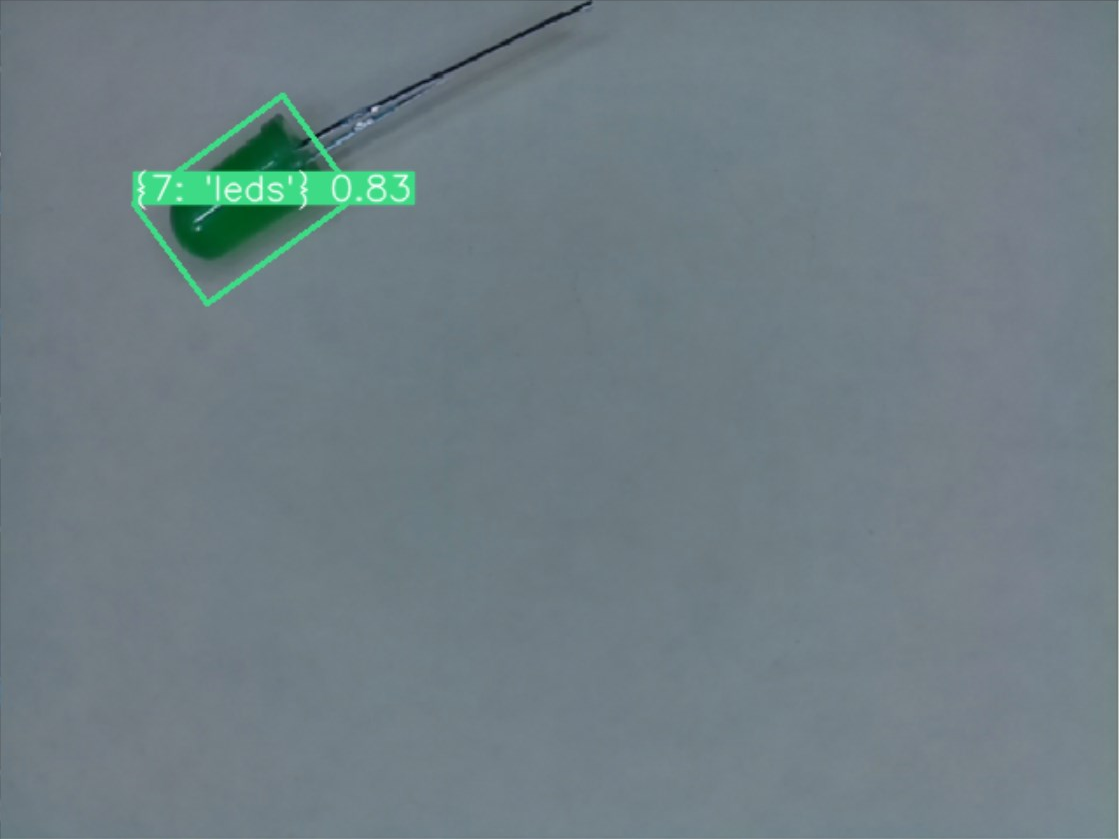
\includegraphics[width=\textwidth]{imgs/cv/2024-05-21_13-04-03_python.jpg}
  \end{minipage}
  \hfill
  \begin{minipage}{0.49\textwidth}
      \centering
      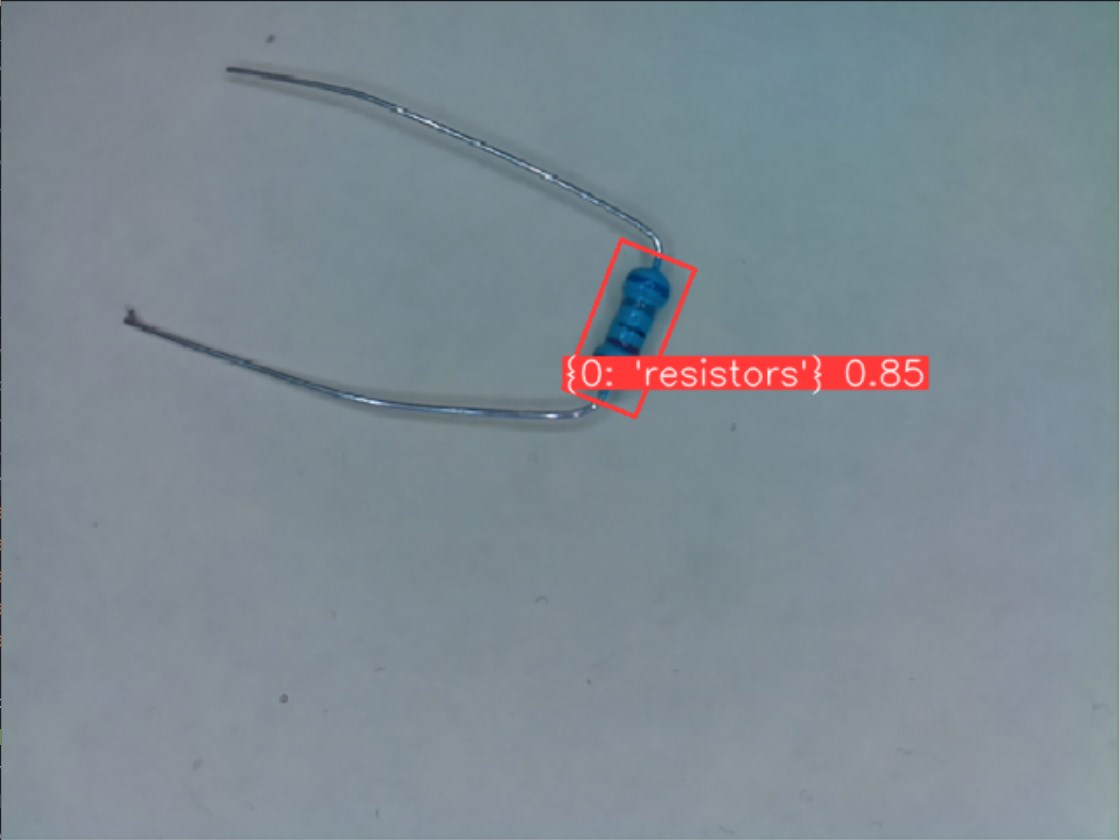
\includegraphics[width=\textwidth]{imgs/cv/2024-05-21_13-04-06_python.jpg}
  \end{minipage}
  \par\medskip
  \begin{minipage}{0.49\textwidth}
    \centering
    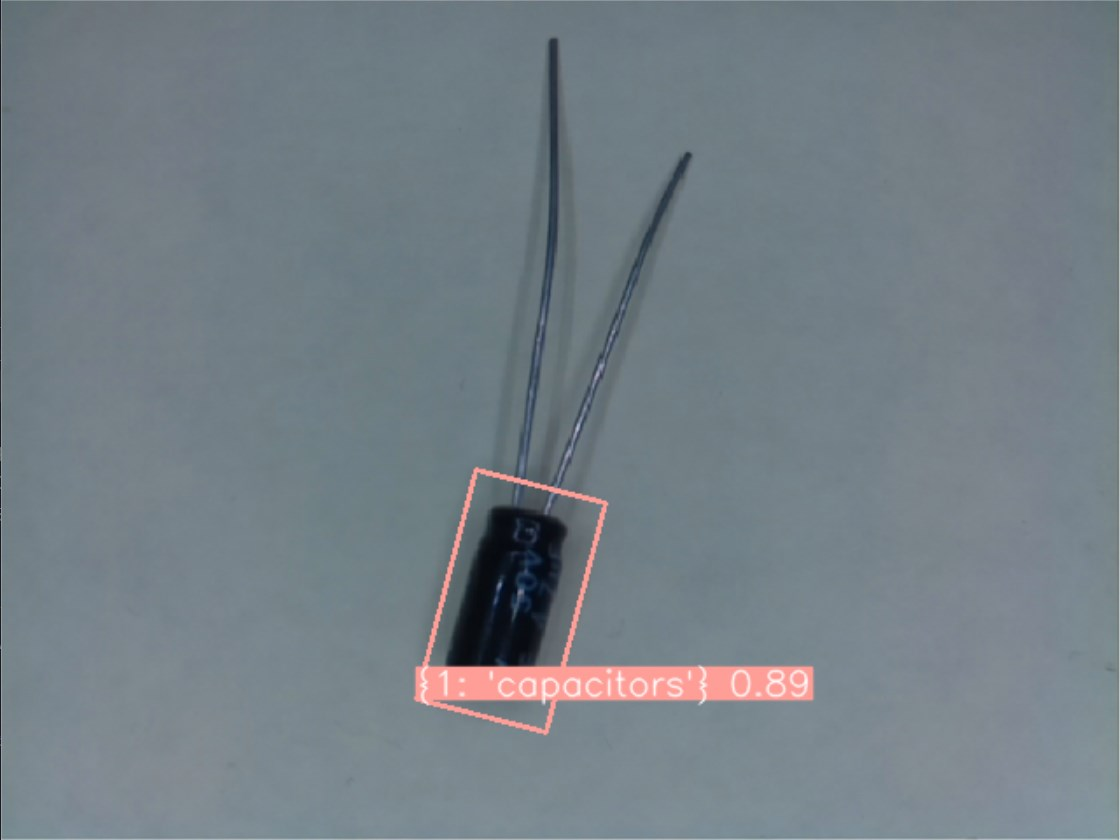
\includegraphics[width=\textwidth]{imgs/cv/2024-05-21_13-04-10_python.jpg}
  \end{minipage}
  \hfill
  \begin{minipage}{0.49\textwidth}
    \centering
    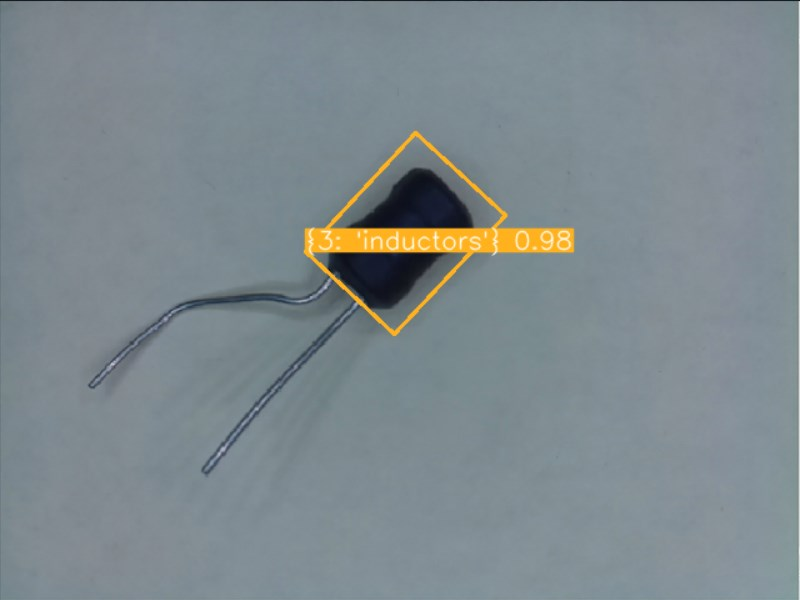
\includegraphics[width=\textwidth]{imgs/cv/2024-06-10_20-47-34_python.jpg}
  \end{minipage}
  \caption{Inference ran using the \texttt{detection-trainer.ipynb} notebook, showing an LED, a resistor, capacitor and inductor, being correctly detected and classified.}
  \label{fig:inference-components}
\end{figure}

For greater clarity, the accuracy of the above inferences are shown in the following table:
\begin{table}[H]
  \centering
  \begin{tabularx}{0.9\textwidth}{|X|X|X|}
    \hline
    \textbf{Component} & \textbf{Confidence} & \textbf{Class} \\
    \hline
    LED & 83\% & LED \\
    \hline
    Resistor & 85\% & Resistor \\
    \hline
    Capacitor & 89\% & Capacitor \\
    \hline
    Inductor & 98\% & Inductor \\
    \hline
  \end{tabularx}
\end{table}

Clearly, the YOLO-OBB model is able to identify and classify the components with a high degree of accuracy with tight, properly oriented bounding boxes. The model is also able to detect components at different orientations and scales, and is able to detect multiple components in the same image. A comprehensive evaluation is conducted in \autoref{sec:computer-vision-evaluation}.

\subsubsection{Component Value Identification}
\label{sec:component-value-identification}
While the YOLOv8-obb model can identify components, it cannot determine the value of the component, for example the resistance of a resistor or the capacitance of a capacitor. 

Originally, the plan was to use the YOLO-OBB model to properly orient the component so that they could be passed into another model for value identification. For regular components, like ceramic capacitors, the value is printed on the component in a standard format, which can be read using OCR (Optical Character Recognition) models and some image preprocessing. However, for resistors, the value is encoded in the colour bands on the resistor, which are relatively small. For this reason, a regular YOLO model was trained to detect and classify colour bands on resistors, and then determine the value of the resistor programmatically, as done in the resistor band data annotation tool discussed in \autoref{fig:resistorannotate}.

\subsubsection{Resistor Value Detection}
\label{sec:resistor-value-detection}
In order to generate the images for the resistor value detection model, the model from the previous section was used to detect the resistors in the images. The generated bounding boxes were then used to crop the images and generate a dataset of resistor images, which were already labelled with the resistor values as explained in \autoref{sec:dataset-collection}.

\begin{figure}[H]
  \hfill
  \begin{minipage}[t]{\textwidth}
    \centering
    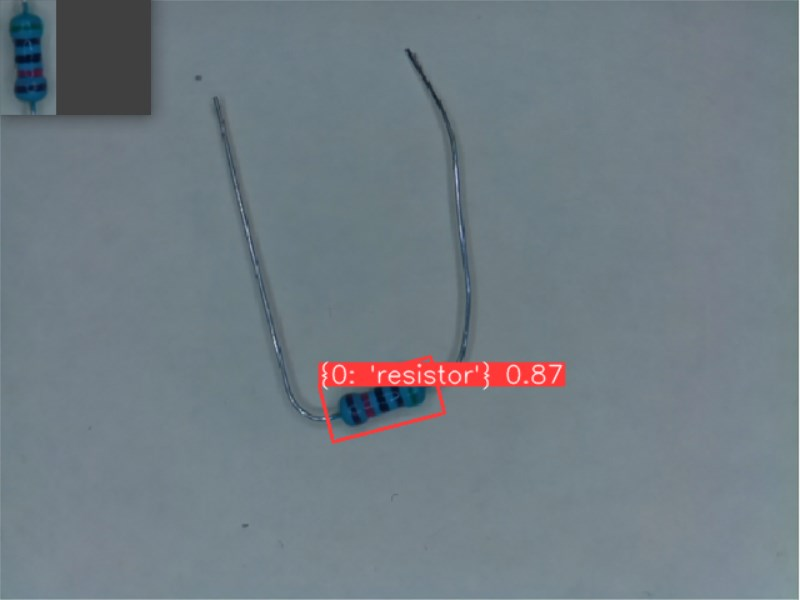
\includegraphics[height=8cm]{imgs/cv/2024-06-10_21-45-23_python.jpg}
    \caption{Resistor Identification and Cropping}
    \label{fig:resistor-cropping}
  \end{minipage}
\end{figure}

As shown in \autoref{fig:resistor-cropping}, a small window opens up that shows the cropped resistor image using OpenCV \cite{home_2024}. The images were then saved to a folder structure matching \autoref{code:dataset-structure}, allowing the resistor value detection model to be trained.

Similiar to the component identification model, the resistor value detection model made use of a 
\\ \texttt{resistor\_trainer.ipynb} notebook that handled the organisation of the dataset, the training of the model, the evaluation of the model, and the ability to run inference on the test set. The notebook also automatically saved the best model weights and leveraged the TensorBoard support that YOLOv8 provides to visualise the training process.

\begin{figure}[H]
  \hfill
  \begin{minipage}[t]{\textwidth}
    \centering
    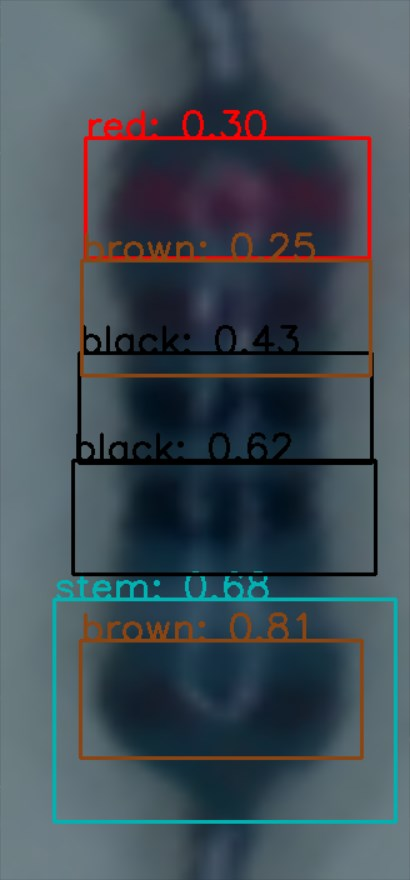
\includegraphics[height=8cm]{imgs/cv/banddetection.jpg}
    \caption{Resistor Band Detection}
    \label{fig:band-detection}
  \end{minipage}
\end{figure}

\subsubsection{Sparsification and Deployment}
\label{sec:sparsification-deployment}
Unfortunately, although SparseML is an incredibly powerful tool, it is not yet compatible with the YOLOv8-OBB model; usually, the SparseML framework integrates with Ultralytics' YOLO models, providing a wrapper that neatly allows sparsification to happen with minimal effort, however sparsification from scratch requires that the optimiser be exposed and a manual training and validation loop be written. This would be possible, however the YOLOv8-OBB model does not expose the optimiser during training, so it would be necessary to rewrite the training loop from scratch, and given the complexity of having to manage the three seperate losses (classification, bounding box, and dfl loss), this would be a significant amount of work. Given the time constraints of the project, it was decided that the model would not be sparsified. This was one of the major design decisions that was made during the project due to the OBB model only being released in January 2024 \cite{obbrelease}, after the Background Research phase had been completed. 

However, although sparsification through SparseML was not possible, the model can still be pruned to achieve a similar effect. Pruning is the process of removing weights from the model that are close to zero, and can be done using the PyTorch pruning library. The model can be pruned to a certain sparsity level, and then fine-tuned to recover the lost accuracy. However, anecdotal evidence seems to suggest that the manual pruning of the YOLOv8 models causes the models to have a slower inference time \cite{pruning}. This could be due to YOLO's complex and efficient architecture, making use of parallel computation and residual connections to speed up inference time \cite{yolo}. Pruning the model could disrupt this architecture, and cause the model to be less efficient.

Despite this, DeepSparse \cite{deepsparse} is still a viable deployment runtime for the model. As discussed in \autoref{sec:background}, the model does not need to be sparsified as a prerequisite for deployment, and can be deployed directly to DeepSparse, albeit without the benefits of sparsification. In \autoref{sec:inference-latency-evaluation}, the model is deployed to DeepSparse and the inference latency is evaluated.

